% +++
% latex="texfot lualatex-dev"
% +++
\documentclass[body]{subfiles}
\begin{document}
\chapter{実験結果}

実験結果(図を貼る)。

\section{\(S=1366\hmu{W/m^2}\)の結果}
地表面温度、子午面温度分布、東西風、時系列

\section{??? の太陽定数依存性}

\section{南北熱輸送の太陽定数依存性}

\(\bullet'=\bullet-\bar\bullet\)、\(\bullet^*=\bullet-[\bullet]\)、
\(\bar\bullet\) は時間平均、\([\bullet]\) は東西平均

\begin{align*}
	[\overline{xv}]&=[\overline{xv}]-[\bar x\bar v]+[\bar x][\bar v]+[\bar x\bar v]-[\bar x][\bar v]\\
	&=[\overline{xv}-\bar x\bar v]+[\bar x][\bar v]+[\bar x\bar v]-[\bar x][\bar v]\\
	&=[\bar x\bar v-\bar x\bar\bar v-\bar\bar x\bar v+\bar\bar x\bar\bar v]+[\bar x][\bar v]
		+([\bar x\bar v]-[\bar x][[\bar v]]-[[\bar x]][\bar v]+[[\bar x]][[\bar v]])\\
	&=[\overline{(x-\bar x)(v-\bar v)}]+[\bar x][\bar v]+[\overline{(x-[x])}\overline{(v-[v])}]\\
	&=[\overline{x'v'}]+[\bar x][\bar v]+[\bar x^*\bar v^*]
\end{align*}

\begin{figure}[t]
	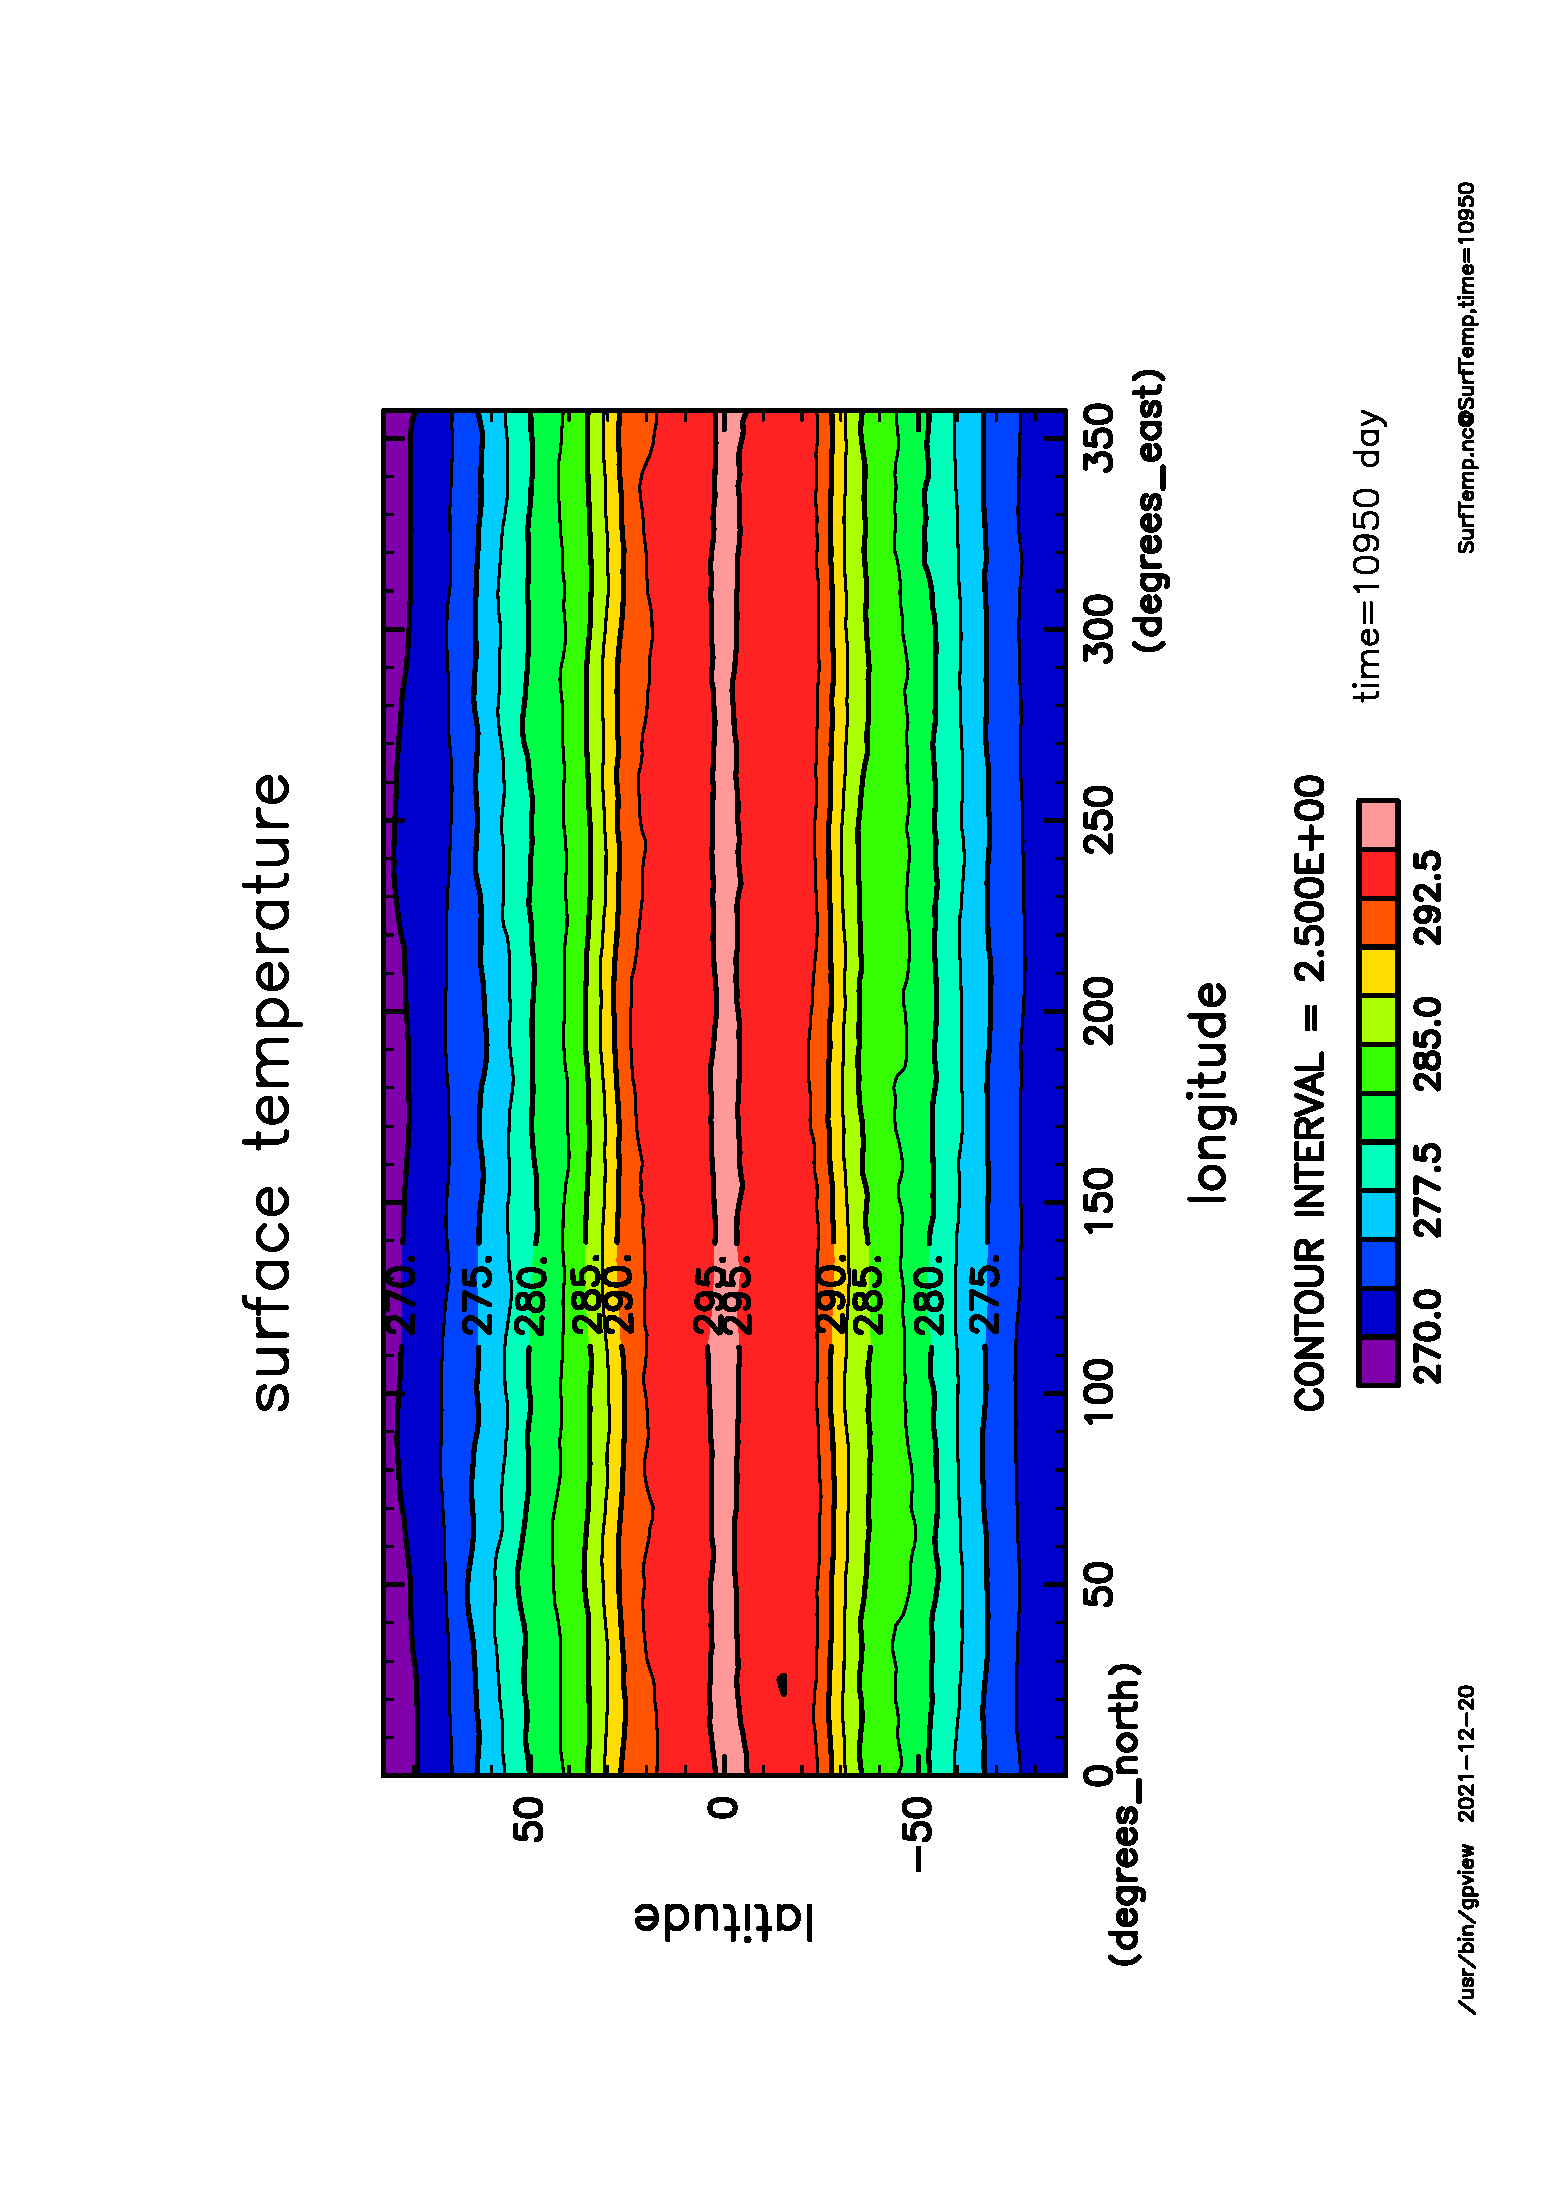
\includegraphics[height=\textwidth,angle=-90]{S1366SurfTemp,time=10950.pdf}
	\caption{\(S=1366\hmu{W/m^2}\) 30 年目の地表面温度}
\end{figure}
\end{document}
